(\textit{Exercise 10.8 S\&B})
The pseudocode in the box on page 251 updates $\bar R_{t}$ using $\delta_{t}$ as an error rather than simply $R_{t+1} -  \bar R_t$.
Both errors work, but using $\delta_{t}$ is better.
To see why, consider the ring MRP of three states from Exercise 10.7.
\begin{figure}
  \center
  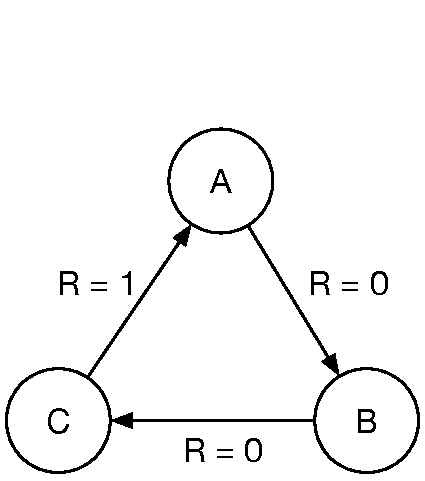
\includegraphics[width=0.2\linewidth]{figures/10dot8.pdf}
\end{figure}
The estimate of the average reward should tend towards its true value of $\frac{1}{3}$.
Suppose you fix $\bar R_{t} = \frac{1}{3}$ and fix $v_{\pi}(A) = \frac{-1}{3}, v_{\pi}(B) = 0, v_{\pi}(C) = \frac{1}{3}$, which are the true values.
What is the sequence of $R_{t+1} - \bar R_{t}$ errors, when going from A to B, B to C and then C to A?
Correspondingly, what is the sequence of TD errors? Here, since we use the true values, we have
$\delta_{t} = R_{t+1} - \bar R_{t} + v_{\pi} (S_{t+1}) - v_\pi (S_{t})$. 
What does this tell us about which error sequence would produce a more stable estimate of the average reward if the estimates were allowed to change in response to the errors? Why?
